\section{数据通信模型}

通信，说到底是一件很古老的事。烽火台、驿站、旗语——人类一直在解决同一个问题：如何把信息从一个地方送到另一个地方，并且让对方能够正确理解。现代数据通信本质上并没有超越这个问题，只是解决它的手段变得极为精妙。

\subsection{从直觉到模型}

设想你要把一段视频发给远方的朋友，中间会发生什么？

首先遇到的是\textbf{内容问题}：视频文件可能有几个GB，直接发送代价高昂。解决方案是压缩——H.264 或 H.265 编码器能将视频压缩到原来的百分之一甚至更小，去掉帧间冗余和人眼不敏感的细节。这是\textbf{信源编码}的任务：提高信息传输的有效性。

然后是\textbf{信道问题}：数据要经过什么"路"传过去？电缆、无线电波、光纤都是可能的选择，每种媒体有不同的特性和代价。更重要的是，媒体不是理想的——噪声、干扰、衰减无处不在，数据在途中会发生错误。因此需要\textbf{信道编码}：加入冗余，让接收方能够发现并纠正错误，以可靠性换取信道利用率。

最后，发送之前还需要\textbf{调制}：把数字信号变换成适合在特定媒体上传输的波形。家里路由器发出的 2.4 GHz 无线电波、海底光缆中的激光脉冲，都是调制的产物。

这三个步骤——信源编码、信道编码、调制——加上它们的逆过程，构成了数据通信系统的基本骨架。Shannon 在 1948 年的论文《通信的数学理论》中将这一骨架形式化，奠定了整个通信理论的基础。

\subsection{通信系统的一般模型}

\begin{figure}[htbp]
    \centering
    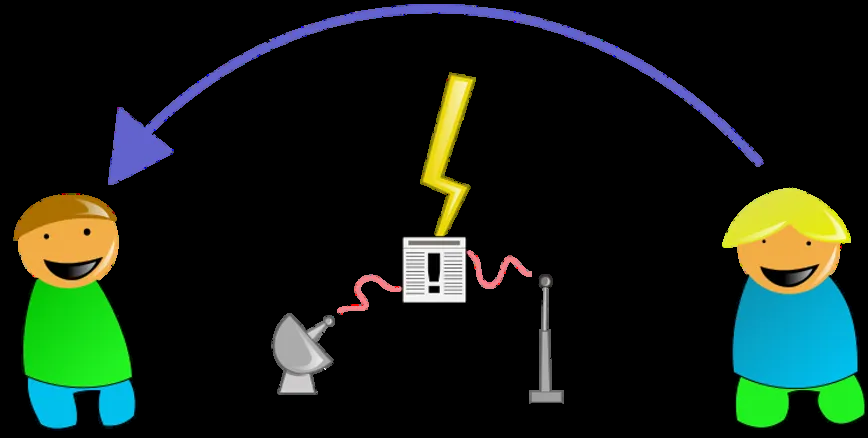
\includegraphics[width=0.9\textwidth]{../assets/ch02/ch02-2_1_数据通信模型-000.png}
    \caption{通信系统一般模型。信源产生的消息经信源编码、信道编码、调制后进入信道传输；接收端经解调、信道译码、信源译码后恢复原始消息。噪声在信道中叠加，是差错的主要来源。}
    \label{fig:comm-model}
\end{figure}

模型的各个部分功能如下：

\textbf{信源（Source）}是消息的产生者。它可以是麦克风（产生模拟语音信号）、摄像头（产生视频流）或键盘（产生数字数据）。从通信系统的角度，信源的输出只有两类：模拟信号和数字信号。

\textbf{信源编码器（Source Encoder）}的任务是压缩：去掉信源输出中的冗余，用尽量少的比特表示信息。ZIP 压缩、JPEG 图像、MP3 音频都是信源编码的例子。没有信源编码，互联网的带宽会在几秒内被耗尽。

\textbf{信道编码器（Channel Encoder）}的任务恰好相反——\textit{增加}冗余。但这些冗余是有结构的，目的是让接收方能从被噪声破坏的信号中恢复出正确的数据。奇偶校验、CRC、汉明码、Turbo 码、LDPC 码都是信道编码的例子。

\textbf{调制器（Modulator）}将数字比特流转换为适合在信道中传输的物理信号。不同的信道需要不同的调制方式：电话线上用 QAM 调制，Wi-Fi 用 OFDM，光纤用 OOK 或 PAM4。

\textbf{信道（Channel）}是传输媒体加上它引入的一切干扰。信道不仅传递信号，也会引入噪声（随机的热噪声）、干扰（其他信号的叠加）和失真（信号波形的畸变）。噪声源在模型中显式标出，提醒我们可靠传输从来不是免费的。

\textbf{接收端}是发送端的镜像：解调器、信道译码器、信源译码器依次恢复出原始消息，最终到达信宿（Sink）——扬声器、屏幕或存储设备。

\subsection{模拟通信与数字通信}

按照信道中传输的信号类型，通信系统分为模拟通信和数字通信。

\textbf{模拟通信}用连续变化的信号（如电压随时间的连续变化）携带信息。传统有线电话就是典型例子：声波推动麦克风膜片振动，转换为连续变化的电流，在铜线上传输，到达接收端再还原为声波。

\textbf{数字通信}用离散的信号（通常是两个电平的序列，即0和1）携带信息。现代通信系统几乎都是数字的。

数字通信为什么能取代模拟通信？根本原因是\textbf{再生中继}。模拟信号每经过一段传输，噪声就会叠加；信号放大时，噪声一并放大，积累下去，质量越来越差。数字信号则不同——接收端不需要精确测量信号的幅度，只需判断它是"高"还是"低"。只要信噪比足够好，接收端就能完美地重建出干净的数字信号，不带任何噪声地继续传递。这就是数字通信的"再生"特性，它让长距离、高质量的通信成为可能。

\begin{figure}[htbp]
    \centering
    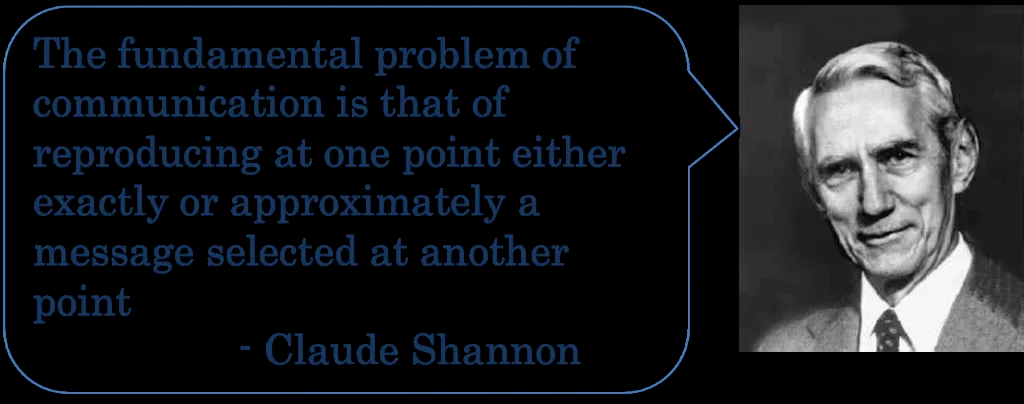
\includegraphics[width=0.85\textwidth]{../assets/ch02/ch02-2_1_数据通信模型-002.png}
    \caption{模拟信号与数字信号的对比。模拟信号（上）幅度连续变化，噪声叠加后无法分离；数字信号（下）只有有限个离散电平，通过阈值判决可以完美再生，噪声不会积累。}
    \label{fig:analog-vs-digital}
\end{figure}

当然，数字通信也有代价：同样的信息，数字化后通常需要更宽的带宽。一路模拟电话只需 4 kHz 带宽，而未压缩的数字电话（PCM）需要 64 kbps，等效于更宽的频带。但随着压缩技术的成熟和光纤带宽的爆发，这一代价已几乎可以忽略。

\subsection{通信方式：单工、半双工与全双工}

点对点通信按数据流向分为三种方式：

\textbf{单工（Simplex）}：数据只能单向流动。广播电台、遥控器是典型例子——发送方永远发，接收方永远收，方向固定。

\textbf{半双工（Half-duplex）}：双方都能收发，但不能同时进行。对讲机是经典案例，说话时按下按钮，释放后才能听到回应。早期的以太网（总线型，CSMA/CD）也是半双工——同一时刻只有一台主机能发送数据。

\textbf{全双工（Full-duplex）}：双方可以同时收发。电话通话是全双工的，你说话的同时对方也能插嘴。现代以太网交换机上的每条链路都是全双工的，消除了冲突，大幅提升了利用率。

\begin{figure}[htbp]
    \centering
    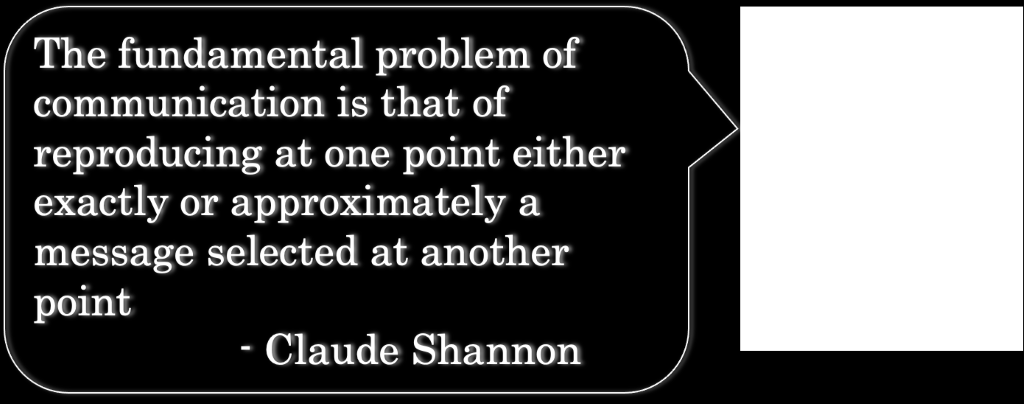
\includegraphics[width=0.8\textwidth]{../assets/ch02/ch02-2_1_数据通信模型-003.png}
    \caption{三种通信方式示意图。(a) 单工；(b) 半双工：同一信道交替使用；(c) 全双工：通常需要两条独立信道（或频分/时分复用的双向信道）。}
    \label{fig:duplex-modes}
\end{figure}

\subsection{数字通信系统模型}

数字通信系统在一般模型的基础上更加明确地展示了各个功能模块：

\begin{figure}[htbp]
    \centering
    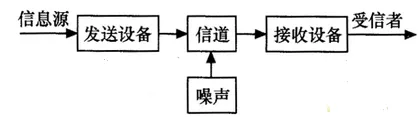
\includegraphics[width=0.95\textwidth]{../assets/ch02/ch02-2_1_数据通信模型-004.png}
    \caption{数字通信系统模型。信源输出经过 A/D 转换（若为模拟信源）、信源编码（压缩）、加密、信道编码（纠错）、数字调制后进入信道；接收端逆向恢复。各模块功能独立，便于单独设计和优化。}
    \label{fig:digital-comm-system}
\end{figure}

值得注意的是\textbf{加密模块}的位置：它在信源编码之后、信道编码之前。这不是随意安排——信源编码后的数据已经被压缩，冗余极少，此时加密效果最好；而信道编码需要在加密后进行，以确保纠错码的保护覆盖加密后的密文（否则信道错误会在解密后产生错误扩散）。

\subsection{从模型到网络}

上述模型描述的是点对点的单向通信。现实中的通信系统是\textbf{网络}——多个节点、多条链路、多种协议交织在一起。点对点的模型是理解网络的基础，但网络带来了新问题：

如何在多个节点之间寻找路径？数据太多时如何排队和调度？多个用户如何共享同一条信道？发生错误或拥塞时如何恢复？这些问题将在后续章节中展开。通信系统一般模型的意义在于：无论网络多复杂，每一条链路、每一个节点上发生的事情，都可以用这个模型来理解。
